\section{Requirements}

Being a project that was experimental in style, the requirements were not
rigidly determined in fine detail at the outset, or even at later stages.
However it was certainly possible, and indeed important, to establish a set of
high-level requirements and guiding principles for the project. These were
categorised as functional and non-functional requirements.

\subsection{Functional Requirements}

The following were regarded as basic features of the program's operation.
\begin{itemize}
\item The program must take a Scheme program as input and produce a Lua program
as output.
\item When the Lua output from the program is run through a Lua interpreter, it
must produce the same output as the Scheme program run natively through a Scheme
interpreter.
\end{itemize}
\begin{framed}
Thinking of the eventual program output raises an interesting question: should
the output ultimately look like Scheme data, or equivalent Lua data?  The answer
to this involves another question around the program's use: is the translator
to be used as a novel interpreter for Scheme, or as a way of constructing
independent Lua programs from Scheme ones? In a role as a kind of Scheme
interpreter, the automatic choice would be to use Scheme data, but perhaps a
translator in the truest sense should output only Lua data.

After consideration, it was decided that the translator output should exactly
match the Scheme output, mainly because this allowed direct comparison of output
with a native Scheme interpreter, which simplified testing. As will be seen
later, it turns out that changing the format of the output to look like Lua is a
trivial matter in any case.
\end{framed}

\subsection{Non-functional Requirements}

Along with the primary functions of the translator, the following had a
significant bearing on the design.
\begin{itemize}
\item The running time of the resulting Lua program should be as short as
possible.
\item The output of the program should be readable Lua code as much as possible.
\end{itemize}

Despite being rather broad, the requirements provided a sound starting point to
work from, influencing design decisions at all stages. In particular the
non-functional requirements, though in possible conflict with each other to a
certain extent, pointed to simplicity as a primary design objective. As an
additional principle, interesting and potentially unusual aspects of the
interactions between the languages were to be given preference over maximal
coverage of the Scheme syntax.


\section{Design 1}

In essence, the translator has a lot in common with an interpreter or a
compiler, insofar as it involves scanning and parsing source code, and
generating output. A simplistic way of looking at it is as a Scheme compiler,
whose output is Lua source code instead of machine code. Because of this, some
of the design decisions were standard, particularly regarding the structure and
main components.

An element of the design that was discussed at the meetings early on, in keeping
with the objective of simplicity, was to try to limit it to a single pass over
the Scheme source files. In that regard, the program would be able to translate
on-the-fly, and therefore could be used in a piped or streamed context. It would
also eliminate the need to build symbol tables, parse trees or other structures.
The uniformity and recursive nature of Scheme's syntax meant that this should be
possible, with the option for multiple passes remaining open if the single pass
wasn't working. In fact, this became the cornerstone of the design and resorting
to multiple passes was not seriously considered at any point.

Given that, the design of other elements of the translator evolved over the
course of the project. Some of the problems encountered forced changes in the
design to varying degrees. In particular, there was one recurring issue, midway
through the project, that prompted a radical redesign of the way the program
handled data.

\subsection{First Approach}

The initial approach involved finding for each construct in Scheme, its most
concise and efficient representation in Lua. In French parlance, this is sweetly
described by the phrase ``le mot juste'', meaning ``the precise word'' or ``the
perfect word'', and it brings to mind the image of an expert translator of
human languages, who knows through experience how to accurately convey the
intended semantic of each phrase from one language to another for a particular
context. At first, this seemed like a reasonable way of proceeding given the
small size of the core of the Scheme language. As well as that, it was the
natural way given that both languages were also being learned together from the
start.

\begin{framed}
For example:
\begin{center}\ttfamily (define identity (lambda (x) x))\end{center}

would be translated to:
\begin{center}\ttfamily identity = function (x) return x end\end{center}
\end{framed}

This method had a number of favourable characteristics like simplicity,
conciseness and readability. The size of the Lua output was minimal, with an
(almost) one-to-one mapping between the Scheme and Lua constructs. Also, all
Scheme atomic data in the input was directly mapped to Lua atomic data, and
Scheme lists were directly mapped to Lua tables.

For now, we will look in more detail at parallels and divergences between the
language elements, before revisiting the design later in the chapter.


\section{Language Elements}

The ability to successfully perform a translation in any setting is affected by
the expressiveness of the languages, particularly the destination language. In
this case, it needed to be determined to what extent the features of Scheme
could be correctly expressed in Lua, both in terms of data representation and
the flow of execution.

\subsection{Data Types}

Scheme data is made up of the following
types:~\cite[Appendix~(Formal~Syntax)]{tspl}
\begin{itemize}
\item \textsc{Atomic Data}: Symbols, Booleans, Numbers, Characters and Strings.
\item \textsc{Compound Data}: Lists, Vectors and Bytevectors
\end{itemize}

We will look at each of these in turn to identify differences that could affect
Lua's ability to fully represent them.

\subsubsection{Symbols}

Scheme symbols define what can constitute a \emph{word} in the language. They
are relevant in how they apply to identifiers. Here is what two of the texts
have to say about symbols and identifiers.

\begin{quotation}\textbf{Scheme:}
``Keywords, variables, and symbols are collectively called identifiers.
Identifiers may be formed from letters, digits, and certain special characters,
including: \texttt ?, \texttt !, \texttt ., \texttt +, \texttt -, \texttt *,
\texttt /, \texttt <, \texttt =, \texttt >, \texttt :, \texttt \$, \texttt \%,
\texttt \^{}, \texttt \&, \rule{3mm}{0.2mm}, \texttt \~{}, and \texttt @ , as
well as a set of additional Unicode characters.  Identifiers cannot start with
an at sign (\texttt @) and normally cannot start with any character that can
start a number, i.e., a digit, plus sign (\texttt +), minus sign (\texttt -), or
decimal point (\texttt .). Exceptions are \texttt +, \texttt -, and \texttt
\ldots, which are valid identifiers, and any identifier starting with
\texttt{->}.''~\cite[Sec~1.1]{tspl}
\end{quotation}

\begin{quotation}\textbf{Lua:}
``Identifiers in Lua can be any string of letters, digits, and
underscores, not beginning with a digit''~\cite[p.5]{luabook}
\end{quotation}

This immediately indicates a possible problem, since Lua identifiers cannot
accommodate the entire range of possible Scheme identifiers.

\subsubsection{Booleans}

With only two possible values, and a boolean type in each language, this is
easily translated. In Lua, the values are \texttt{true} and \texttt{false},
corresponding to \texttt{\#t} and \texttt{\#f} respectively in Scheme.

\subsubsection{Numbers}

Scheme has a very rich syntax for describing numbers. This is in contrast with
Lua, in which the double precision floating point number is the only
numeric type.

\begin{quotation}\textbf{Scheme:}
``Scheme numbers may be classified as integers, rational numbers, real numbers,
or complex numbers. This classification is hierarchical, in that all integers
are rational, all rational numbers are real, and all real numbers are
complex.''\ldots ``A Scheme number may also be classified as exact or inexact,
depending upon the quality of operations used to derive the number and the
inputs to these operations.''~\cite[Sec~6.4]{tspl}
\end{quotation}

\begin{quotation}\textbf{Lua:}
``The number type represents real (double-precision floating-point) numbers. Lua
has no integer type, as it does not need it.''~\cite[p.10]{luabook}
\end{quotation}

It is clear from this that numbers cannot translate directly, so some other
method of dealing with it would need to be found.

\subsubsection{Characters and Strings}

Lua does not have a specific character type. Scheme characters could potentially
be represented in Lua as a single character string, but this would make them
indistinguishable from an actual single character string. Here is the
information pertaining to strings in Scheme and Lua from the texts:

\begin{quotation}\textbf{Scheme:}
``A string is written as a sequence of characters enclosed in double
quotes,''\ldots ``Any Unicode character may be inserted''~\cite[Sec~6.8]{tspl}
\end{quotation}

\begin{quotation}\textbf{Lua:}
``Lua is eight-bit clean and its strings may contain characters with any numeric
code, including embedded zeros. This means that you can store any binary data
into a string''~\cite[p.11]{luabook}.
\end{quotation}

This indicates that, aside from the previously mentioned issue with characters, strings should be transferrable without much trouble.

\subsubsection{Lists}

Lists are the primary data type in Scheme, and there is a duality in the
representation of list data and the core syntax of a Scheme program.

\begin{quotation}
``The pair, or cons cell, is the most fundamental of Scheme's structured object
types. The most common use for pairs is to build lists, which are ordered
sequences of pairs linked one to the next by the cdr field. The elements of the
list occupy the car fields of the pairs. The cdr of the last pair in a proper
list is the empty list, (); the cdr of the last pair in an improper list can be
anything other than ().''~\cite[Sec~6.4]{tspl}
\end{quotation}


Similarly, Lua has a single, but very flexible data structure called a
\emph{table}, which amounts to an associative array, but with added features
such as meta-methods, allowing it to do numerous things such as object-oriented
programming.
\begin{quotation}
``Tables are the main (in fact, the only) data structuring mechanism in Lua, and
a powerful one. We use tables to represent ordinary arrays, symbol tables, sets,
records, queues, and other data structures, in a simple, uniform, and efficient
way''~\cite[p.14]{luabook}.
\end{quotation}

The power of tables allows many things to be accomplished, and is more than
capable of representing Scheme data lists.


\subsubsection{Vectors and Bytevectors}

Vectors are similar to lists in that they represent a sequence of values, but
they are not conceptually represented in pair form. Bytevectors are a special
type of vector, whose elements represent byte values.
\begin{quotation}
``Vectors are more convenient and efficient than lists for some applications.
Whereas accessing an arbitrary element in a list requires a linear traversal of
the list up to the selected element, arbitrary vector elements are accessed in
constant time.''~\cite[Sec~6.9]{tspl}

``Bytevectors are vectors of raw binary data. Although nominally organized as a
sequence of exact unsigned 8-bit integers, a bytevector can be interpreted as a
sequence of exact signed 8-bit integers, exact signed or unsigned 16-bit,
32-bit, 64-bit, or arbitrary-precision integers, IEEE single or double
floating-point numbers, or arbitrary combinations of the
above.''~\cite[Sec~6.10]{tspl}
\end{quotation} 
As with lists, both vectors and bytevectors could be easily represented using Lua tables.

\subsection{Equality}

Scheme has quite a complex interpretation of equality, with each data type
having multiple degrees of equivalence~\cite[Sec~6.2]{tspl}.
\begin{framed}
For example, the lists \texttt{'(1 2)} and \texttt{(cons 1 '(2))} are considered
the same under the \texttt{equal?} predicate, but not \texttt{eq?}, which
requires the pointer values of both lists to be the same.

Similarly, different predicates give different answers for numbers:
\begin{center}
\ttfamily
\verb|(eqv? 3 3.0) => #f (false)| \\
\verb|(equal? 3 3.0) => #f (false)| \\
\verb|(= 3 3.0) => #t (true)|
\end{center}
\end{framed}
Equality in Lua is not as intricate as this, and this disparity will also need
consideration.

\subsection{Branching}

Both Scheme and Lua contain constructs that allow branching, but they differ in
the way they operate. In Scheme, this can be achieved using \texttt{if},
\texttt{when}, \texttt{unless}, \texttt{case} and \texttt{cond}. Like the rest
of Scheme it is expression-based, meaning that the execution of the branch
instruction amounts to a value of some sort. In contrast, Lua's main branch
instruction, \texttt{if}, is a statement, which does not implicitly have a value
of itself. A simple conditional expression can be formed in Lua using the
\texttt{and} and \texttt{or} operators.

\subsection{Looping}

Looping in Scheme is done using expressions like named \texttt{let},
\texttt{letrec} and \texttt{do}. Lua contains the iterative statements
\texttt{while}, \texttt{for} and \texttt{repeat}, similar to many imperative
programming languages. It can also be used recursively, and is fully
tail-recursive. As with branching, the translation must accommodate the
expression-based form of Scheme.

\subsection{Functions}

Scheme supports defining new functions using \texttt{lambda}, as in Church's
lambda calculus. Lua does so in a C-like style with \texttt{function}. Both
treat functions as first-class values that are inherently anonymous, allowing
great flexibility in their use. In general, Scheme procedures evaluate the
arguments before calling the function, but some special syntaxes, such as
\texttt{and} and \texttt{or}, do not. This could present a problem for the
translator when passing arguments directly to Lua functions, since Lua always
evaluates the function arguments in advance of calling the function.

\subsection{Continuations}

Continuations are a feature of Scheme that do not have an exact parallel in Lua.

``One-shot'' continuations could be implemented using a Lua feature called
coroutines.

\subsection{Syntax Extension}

This is another aspect of Scheme to be considered. It does not have a direct
counterpart in Lua.

\begin{quotation}
``Syntactic extensions, or macros, are used to simplify and regularize repeated
patterns in a program, to introduce syntactic forms with new evaluation rules,
and to perform transformations that help make programs more
efficient.''~\cite[Ch~8]{tspl}
\end{quotation}

An implementation of this would create the potential for the translator to be
able to enhance its own capabilities during translation, which is a very
interesting prospect.


\section{Design 2}

The above considerations naturally had an influence on the design, with the full
extent of their implications taking some time to become apparent. As the
project progressed, and as more functionality was added to the translator, a
number of issues prompted a rethink of some parts of the original design.

\subsection{Difficulties With First Approach}

Number representation, data problems, context problems, identifier mappings,
equality, function arguments.

Here is a very basic example of the problem presented by the context:
\begin{framed}
Take the Scheme expression \texttt{(+ 4 5)}. According to the first approach,
this should be translated as \texttt{4 + 5}. However, if this was a
sub-expression in the larger expression \texttt{(*~3~(+~4~5))}, the result would
be \texttt{3~*~4~+~5}, which is incorrect. The problem is that precedence is
an integral part of the Scheme syntax that was lost in translation in this case.
The obvious solution is to make this explicit in the translation using brackets,
but to do this succinctly requires an intelligence and awareness of the context,
and similar awareness must be applied to all constructs, not just arithmetic
expressions.
\end{framed}
The solution that was applied in this case was, somewhat unfortunately, to
explicitly define the precedence for all contexts. In other words, brackets were
applied to every operand of every arithmetic expression---making the translation
of the above \texttt{(3) * ((4) + (5))}. This is quite difficult to read for
such a small expression. A similar technique had to be applied to functions.

It was possible to delay the evaluation of function arguments using a
\emph{thunk}, which involves wrapping the argument in a function, to be called
if and only if the argument is needed.

However it soon became apparent that this approach would quickly become
unwieldy, as the range of various contexts in which an expression could appear
often meant the optimal translation needed to be adjusted slightly. An example
of this is\ldots

A trade-off emerged between complexity in the translator and the complexity of
the output. In effect, making the output as simple and efficient as
possible would mean a large degree of complexity in the translator,
characterised by constant type checking, monitoring of context, and applying
rules.

\subsection{Second Approach}

\begin{figure}
\centering
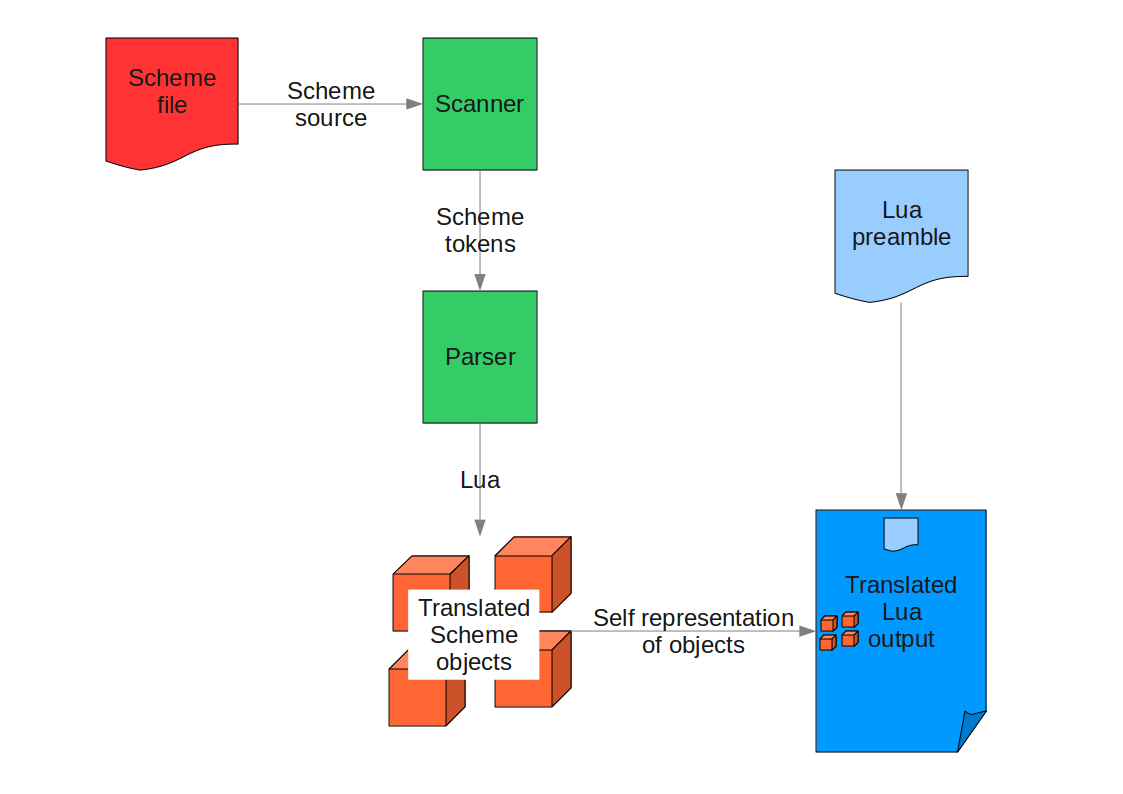
\includegraphics[width=\textwidth]{overview.png}
\caption{A conceptual overview of the stages of translation}
\label{fig:overview}
\end{figure}

This approach was more structured in its implementation, and it attempted to
address some of the problems described above. Figure~\ref{fig:overview} shows
the main concept in pictorial form. The source file would be scanned and parsed
as before. However, instead of directly outputting Lua source, the parser would
represent the Scheme program as a set of data objects, the evaluation of which
would cause them to output themselves as Lua code. Furthermore, every
translation would be preceded by a preamble containing definitions of the data
objects and a library of supported Scheme operations.


\section{Implementation}

The implementation of the translator was incremental, and subject to the design
difficulties described above. The large extent of the redesign hampered progress
on new features, and the initial priority was on simple arithmetic and basic
control operations. This was quite disappointing, but enough was completed to
successfully translate a range of useful Scheme programs, and a good platform is
now there for the more complex and interesting features. Here is a list describing what has been implemented:

\begin{description}
\item[Data Types] Support for vectors and bytevectors was included, but they
were not tested to any great degree.
\item[Assignment, Arithmetic and Comparison] t
\item[Functions] including delayed evaluation of arguments
\item[Branching] t
\item[Looping] t
\end{description}

The following is the list of features yet to be implemented, in order of their
priority. The priority was determined by a combination of how interesting the
feature is, and what would be involved in the implementation.
\begin{description}
\item[Continuations] 
\item[Syntax Extension] 
\item[The Scheme Number Syntax] would not be too difficult with the
structure in place. It would involve expanding the \texttt{scmNumber} data type
to include the necessary attributes and operations.
\item[Equality] could be implemented trivially in an object-oriented manner
by adding the various equality methods to the data types.
\item[Full coverage of Scheme procedures] would be a case of adding a function
to the library for every procedure. Implementing syntax extension could
facilitate this in an interesting way.
\end{description}


\section{Components}

The translator consists of one shell script, one Lua file providing mappings for
Scheme special syntaxes and names, and five Lua files representing the main
components. The source code can be found in Appendix~\ref{sec:sourcecode}. The
following are descriptions of the components and how they operate.

\subsection{Main Program}

The entry point to the translator is a shell script that outputs the preamble
and then calls the main \texttt{scheme2lua.lua} program, which contains the main
loop. It take a number of Scheme input files as arguments and writes the Lua
translation to standard output. The usage is:

\begin{framed}
\texttt{\$ ./scheme2lua [input-file] \ldots}
\end{framed}

The \texttt{scheme2lua.lua} program is a filter, which takes Scheme from its
standard input and outputs Lua to standard output. It does this through a loop
that repeatedly calls the \texttt{parse} function on the next token of input,
until none remain. Algorithm 1 shows the main loop:

\begin{algorithm}
\caption{Main Loop For Translator}
\label{alg:mainloop}
\begin{algorithmic}
\STATE expression $\leftarrow$ parse next token  
\WHILE{expression $\neq$ nil}
\STATE print tostring(expression)
\STATE expression $\leftarrow$ parse next token
\ENDWHILE
\end{algorithmic}
\end{algorithm}

\subsection{The Scanner}

\begin{figure}
\centering
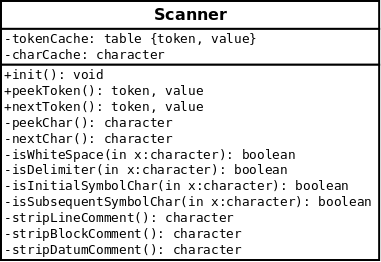
\includegraphics[width=\textwidth]{scannerUML.png}
\caption{A UML class diagram of the scanner component}
\label{fig:scannerUML}
\end{figure}

The scanner component is used to read the input file(s) and split them into a
stream of atomic tokens, which are supplied to the parser. Scanners are a common
component in compilers and interpreters and, rather than attempt to re-invent
the wheel, a standard approach to scanning was followed for this project.
Though it used a slightly different implementation, it was created borrowing
heavily from the ideas and techniques used in the SAL interpreter\cite{sal}.

Figure~\ref{fig:scannerUML} shows the structure of the scanner in UML class
form. As can be seen from the diagram, the scanner is accessible through three
methods: \texttt{init()} initialises the scanner; the others return individual
tokens from the scanner---the difference being that \texttt{peekToken()} leaves
the returned token in the scanner, whereas \texttt{nextToken()} does not.
Internally, there are helper methods and attributes for dealing with caching,
comments and recognising the various Scheme tokens.

\subsection{The Parser}

\begin{figure}
\centering
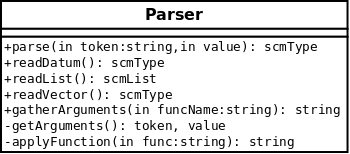
\includegraphics[width=\textwidth]{parserUML.png}
\caption{A UML class diagram of the parser component}
\label{fig:parserUML}
\end{figure}

The parser is at the heart of the program, particularly the parse function,
which does the main work in translation. It has a simple algorithm:
\begin{itemize}
\item When given a token of atomic data, it returns a data object representing
that type and value.
\item If the token is an open list parenthesis, this indicates an imminent
procedure. It recursively parses the next token, interprets that as the
procedure, and applies it using the remaining items in the list as arguments.
\end{itemize}
The parser also has some utility functions for reading compound data and
function arguments from the scanner. See figure~\ref{fig:parserUML} for a UML
representation of the component.

\subsection{The Preamble}

The preamble forms the beginning of the output of every translation. It is
created through the verbatim output of two files, \texttt{dataTypes.lua} and
\texttt{procedures.lua}, which respectively define the data types and procedures
needed by the translated source code.

\subsubsection{Preamble Data Types}

\begin{figure}
\centering
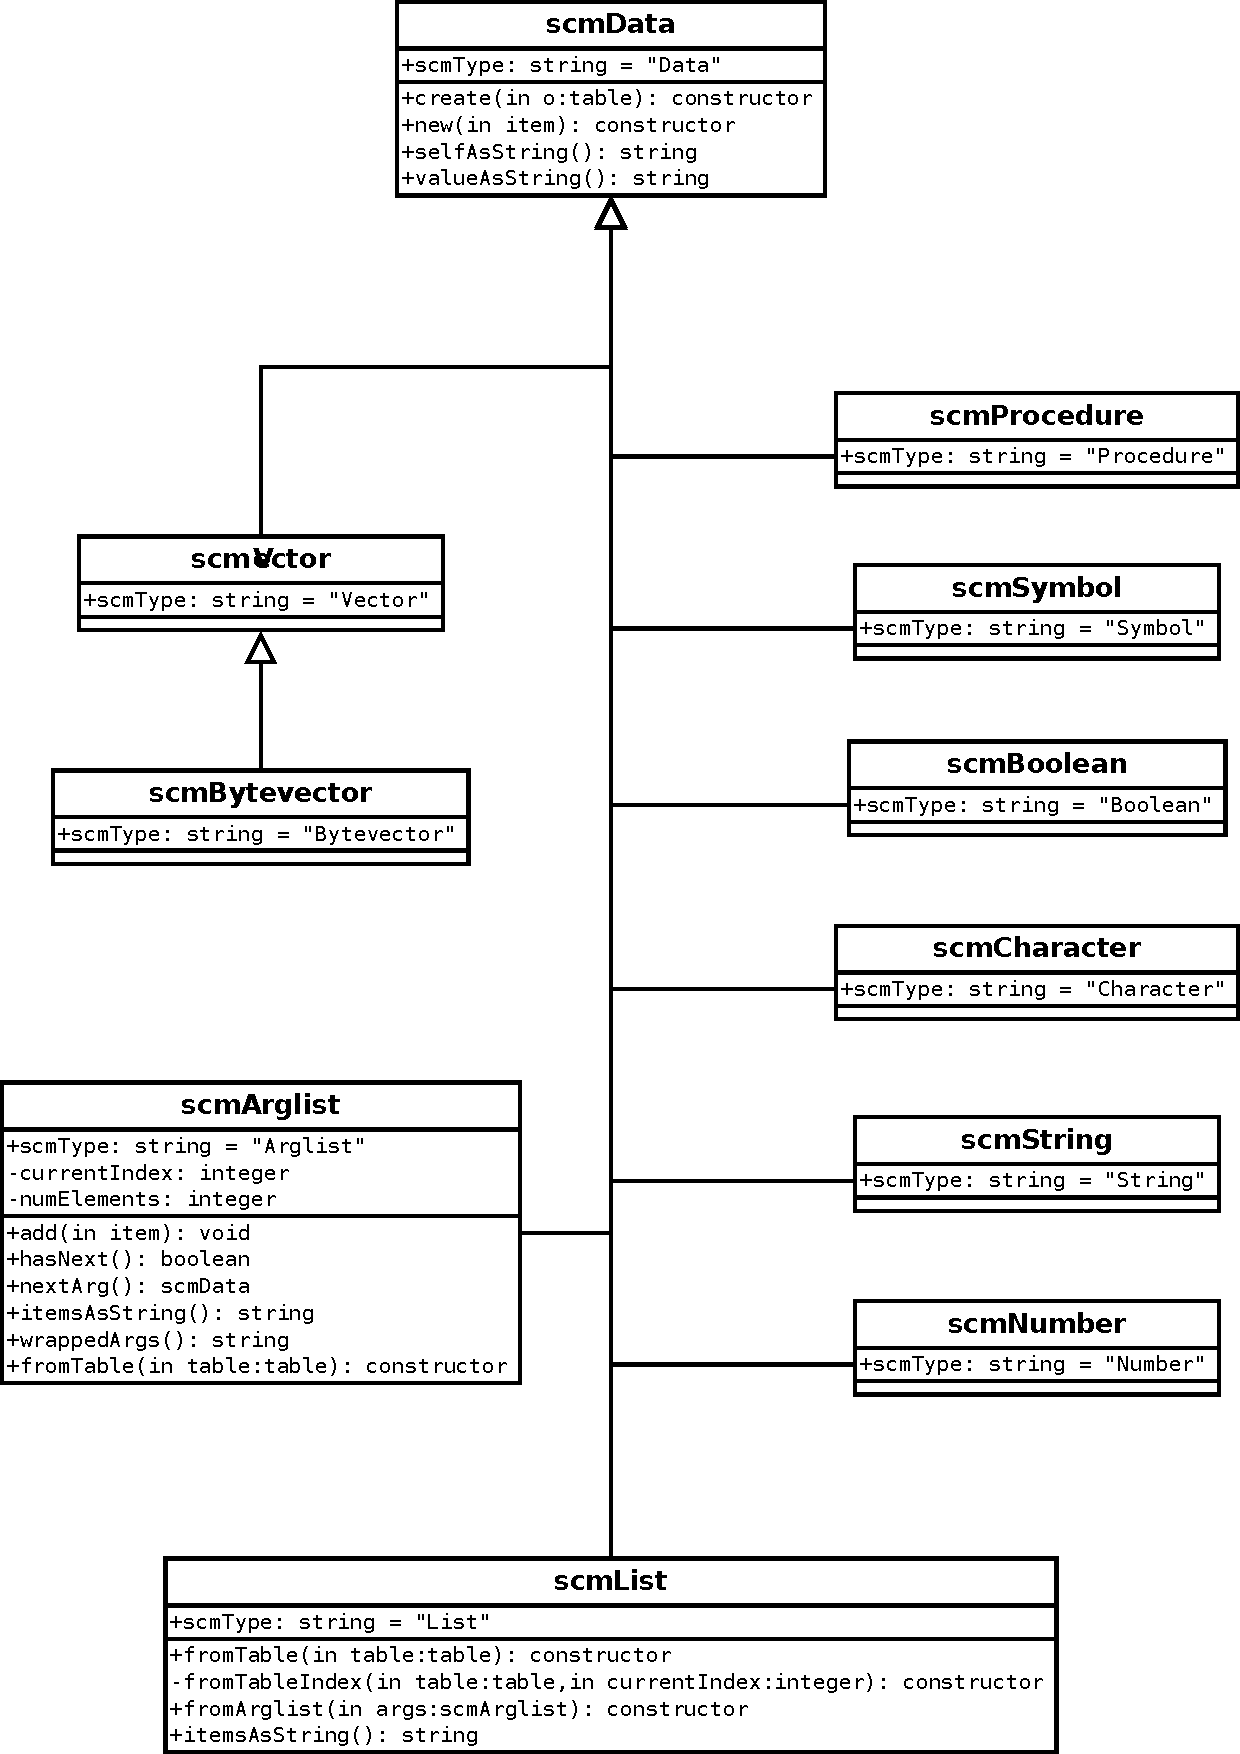
\includegraphics[width=\textwidth]{scmDataUML.pdf}
\caption{The structure of the intermediate data types}
\label{fig:scmDataUML}
\end{figure}

The output of the parser is in the form of intermediate data structures, written
in Lua, representing Scheme data and procedures. They are used both by the
parser and in the resulting Lua program. As a result, they have two
string representations.
\begin{description}
\item \texttt{selfAsString()} is a kind of self-replication function. It
generates the Lua code necessary for the object to create itself.
\item \texttt{valueAsString()} is the string representation of that piece of
data, as expected in the final output.
\end{description}
Furthermore, the \texttt{tostring()} meta-method of each of these data types is
configured to be \texttt{valueAsString()}. This means that changing the
translator output from looking like Scheme to looking like Lua, as mentioned
earlier, is a matter of changing the \texttt{valueAsString()} method for each of
the data types.

Encapsulating the Scheme data in this way has another side-effect. Being
objects, each data type can be enriched with more complex representations and
extra operations as necessary. This provides a way of implementing the more
complex Scheme number syntax.

The structure and relationship between the data types can be seen in
figure~\ref{fig:scmDataUML}.

\subsubsection{Preamble Procedures}

The second part of the preamble is a series of Lua functions that implement the
supported Scheme constructs. This acts as a library to be used by the
translated Scheme source.

All of the functions of the library deal with data in the intermediate form, as
output by the parser. That is to say that all arguments and all return values of
all library functions are in this form. The underlying value can be accessed
using the \texttt{value} attribute, or by calling \texttt{tostring()} on the
data for a string representation, as in the main loop of the program.


\section{The Format Of A Translated Program}

As described above, the output of the translator consists of two main parts:
\begin{itemize}
\item The preamble written in Lua, consisting of the definitions of the
intermediate data structures, and a library of supported Scheme functions and
operations. This is identical for every translation;
\item The translated output of the Scheme program, which uses a subset of the
library to carry out its purpose. This part can contain calls to the library
functions and other output created from Scheme special syntaxes.
\end{itemize}

To conclude this chapter, we will look at an example involving the translation
of the following simple Scheme program, which displays the sum of 1 and 2 on the
screen:
\begin{framed}
\centering
\texttt{(display ((lambda (x y) (+ x y)) 1 2))}
\end{framed}
This is to illustrate the overall format of the output. Consequently, some parts
of the preamble have been omitted for brevity. A complete example can be found
in Appendix~\ref{sec:transexample}.

\begin{framed}
\scriptsize
\begin{verbatim}
--
-- SCHEME TO LUA TRANSLATOR
-- Preamble File 1
-- This file contains lua container tables for scheme data
--
\end{verbatim}
\vdots \textbf{*** Some code omitted ***}\\ \vdots
\begin{verbatim}
--
-- Data type to hold a scheme number
--
scmNumber = scmData:create{
    scmType = "Number";
}
\end{verbatim}
\vdots \textbf{*** Other data definitions omitted ***}\\ \vdots
\begin{verbatim}
--
-- SCHEME TO LUA TRANSLATOR
-- Preamble File 2
-- This file contains the lua implementation of the scheme functions
--

--
-- BEGIN SCHEME FUNCTIONS
--
\end{verbatim}
\vdots \textbf{*** Some functions omitted ***}\\ \vdots
\begin{verbatim}
function s2l_arithmeticPlus(...)
    local result = 0
    for _, item in ipairs{...} do
        result = result + item.value
    end
    return scmNumber:new(result)
end
\end{verbatim}
\vdots \textbf{*** Some functions omitted ***}\\ \vdots
\begin{verbatim}
--
-- END SCHEME FUNCTIONS
--

s2l_display((function (x, y)
return s2l_arithmeticPlus(x, y)
end)(scmNumber:new(1), scmNumber:new(2)))
\end{verbatim}
\end{framed}

The actual translated output is represented by the last three lines, and it uses
the \texttt{scmNumber} data type and two functions from the preamble:
\texttt{s2l\_display} and \texttt{s2l\_arithmeticPlus}. Although quite different
in syntax, there is considerable resemblance between these three lines and the
original Scheme program.
